
% Shorthand since we are not sure about the name of the library yet
\newcommand{\CCLTrackerJS}{ \emph{CCLTracker Javascript Library} }

%%%%%%%%%%%%%%%%%%%%%%%%%%%%%

As mentioned before, \emph{Google Tag Manager} provides a simple, graphical interface for defining analytics events. These events target some particular DOM elements in the website, identified by some characteristics. Providing this information is a trivial task for simple websites, but it's nearly impossible on web applications. That's because there are too many elements to keep track of, and their semantics might even change over time (ex. a 'Start' button might become a 'Stop' button).Therefore we need to have a higher-level information that should come directly from the application. 

There are already various analytics toolkits available, however they are either overly complicated, or they abstract too much information, making it more complicated for us to process the data\footnote{https://segment.com/docs/libraries/analytics.js/}. Moreover, most of these solutions are available only with a paid subscription or not available under an open-source licence. In addition, we didn't want to lose the core functionality from \emph{Google Analytics} or \emph{Piwik}, so we decided to develop an additive solution.

Therefore, we designed the \CCLTrackerJS~\footnote{https://github.com/wavesoft/CCLtracker} to be a set off tools for simplifying the communication with an analytics provider, while in the same time de-decoupling the work of the developer and the analytics expert. The library works as a proxy between the application and the analytics provider, decoupling the tasks of the developer and the analytics expert.

In the following sections we are going to explain in a greater detail how the \CCLTrackerJS works and how it is used in our projects.

%%%%%%%%%%%%%%%%%%%%%%%%%%%%%
%%%%%%%%%%%%%%%%%%%%%%%%%%%%%
\subsection{Technical Details}
%%%%%%%%%%%%%%%%%%%%%%%%%%%%%
%%%%%%%%%%%%%%%%%%%%%%%%%%%%%

Since our goal was to clarify ambiguous events, the web application has to trigger the high-level events when needed. In order to minimise the integration effort, the \CCLTrackerJS takes care of offloading most of the concerns from the developer. Upon loading, events can be triggered right away using the \texttt{analytics.fireEvent(..)} function, without caring about the analytics provider that will receive them. In addition, the library takes care that no events are lost even if the analytics provider becomes available at a later time.

Internally, the \CCLTrackerJS keeps a buffer with all the pending events, and waits for a callback from the analytics provider when it's loaded. To be more precise, the library will wait for a fixed amount of time until a function named \texttt{analyticsListener} is defined in the global scope. When the \texttt{analyticsListener} function is defined, the library will flush all the pending events to the analytics provider and then forward all calls to \texttt{analytics.fireEvent}, to \texttt{analyticsListener}. Even if this function is never defined, the library assumes that the request was blocked due to tracking/ad-blocking extensions in the browser and pauses the analytics collection. 

\begin{figure}[t]
  \begin{center}
		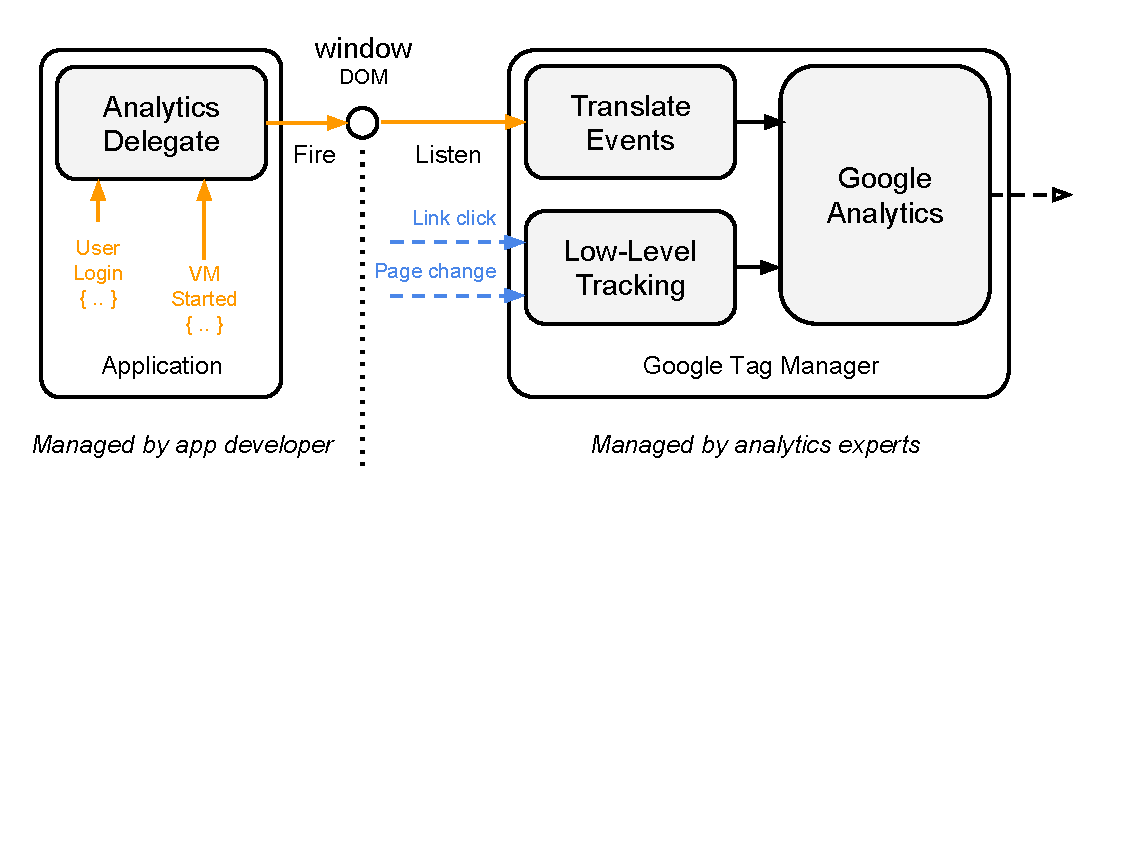
\includegraphics[width=\columnwidth]{imgs/CERN60Events.pdf}
  \end{center}
\caption{Event flow in application using CCLTracker and Google Analytics. The \CCLTrackerJS is the \emph{Analytics Delegate}, on the left}
\label{fig:cern60events}
\end{figure}

There are two different methods for fording the events to the provider: 
\begin{itemize}
\item Through a \textbf{drain function}, that will receive every event being produced, or
\item Through \textbf{event-binding} using the DOM Window as a proxy element.
\end{itemize}

The second method is favoured in our case, since the analytics logic is managed by the analytics experts and is delivered through Google Tag Manager (GTM). The developer creates a specification document describing all the events triggered by the application, and analysts use GTM to listen for particular events in the window DOM. This way, developers expose all the information required to accurately describe an event, and analysts decide to how and what is going to be processed.  

This approach is also illustrated in Figure~\ref{fig:cern60events}. The application triggers events to the \CCLTrackerJS, which get forwarded to the code provided by the analytics experts through GTM. The big benefit of this approach is the fact that additional events, that were not previously accounted for, can be tracked using the low-level tracking features of GTM or any other tracking provider.

%%%%%%%%%%%%%%%%%%%%%%%%%%%%%
\subsubsection{Persistent Store}
%%%%%%%%%%%%%%%%%%%%%%%%%%%%%

In one of our complicated examples, in the \emph{CERN 60 Computing Challenge}, it was important for us to preserve the state across browsers or sessions. That's because the user was instructed to start a Virtual Machine and we wanted to count how many hours (s)he spent on it. Our solution was to check the state of the machine every time the user comes back to the interface and if the VM is still running, accumulate the time since the last check. However, this introduced a problem, since we could not preserve the state information across different browsers.

To solve this problem, \CCLTrackerJS is equipped with a state sharing mechanism. Thus, when the state of the library is changed, a callback is fired, allowing interested parties to push the change to a persistent store. Likewise, it provides an \texttt{importStore} function for importing a previously archived state. 

In the case of CERN 60 Computing Challenge we maintained the persistent store as custom VM property, accessible through the \emph{CernVM WebAPI}~\footnote{https://github.com/wavesoft/cernvm-webapi/} library. When a browser window is focused the analytics store is restored from the VM property and when a change occurs gets immediately committed back.

%%%%%%%%%%%%%%%%%%%%%%%%%%%%%
%%%%%%%%%%%%%%%%%%%%%%%%%%%%%
\subsubsection{Usage Examples}
%%%%%%%%%%%%%%%%%%%%%%%%%%%%%
%%%%%%%%%%%%%%%%%%%%%%%%%%%%%

TODO


%
%\begin{itemize}
%\item What is CCLTracker JS library?
%\item What is the contribution of using CCLTraker library compared with starting a implementation from scratch. 
%\item Technical description of the Library
%\item Setting up the library, requirements, scope,...
%
%\end{itemize}
%

%\subsubsection{Description of the events}
%
%The tracking is implemented via high-level events fired by the Challenge interface, which are then collected and forwarded to the Google Analytics. There are two major categories of events:
%
%Related to CernVM WebAPI 
%Related to user actions
%
%The events fired to the DOM window are always prefixed with the ‘analytics.’ prefix.
%
%\subsubsection{CernVM WebAPI Events}
%
%Most of the CernVM WebAPI events are fired when the state of the internal finite-state-machine is changed. For reference, the following abstract diagram illustrates the different states in the internal FSM and the possible transitions between them:
%
%
%
%\begin{figure}[t]
%  \begin{center}
%		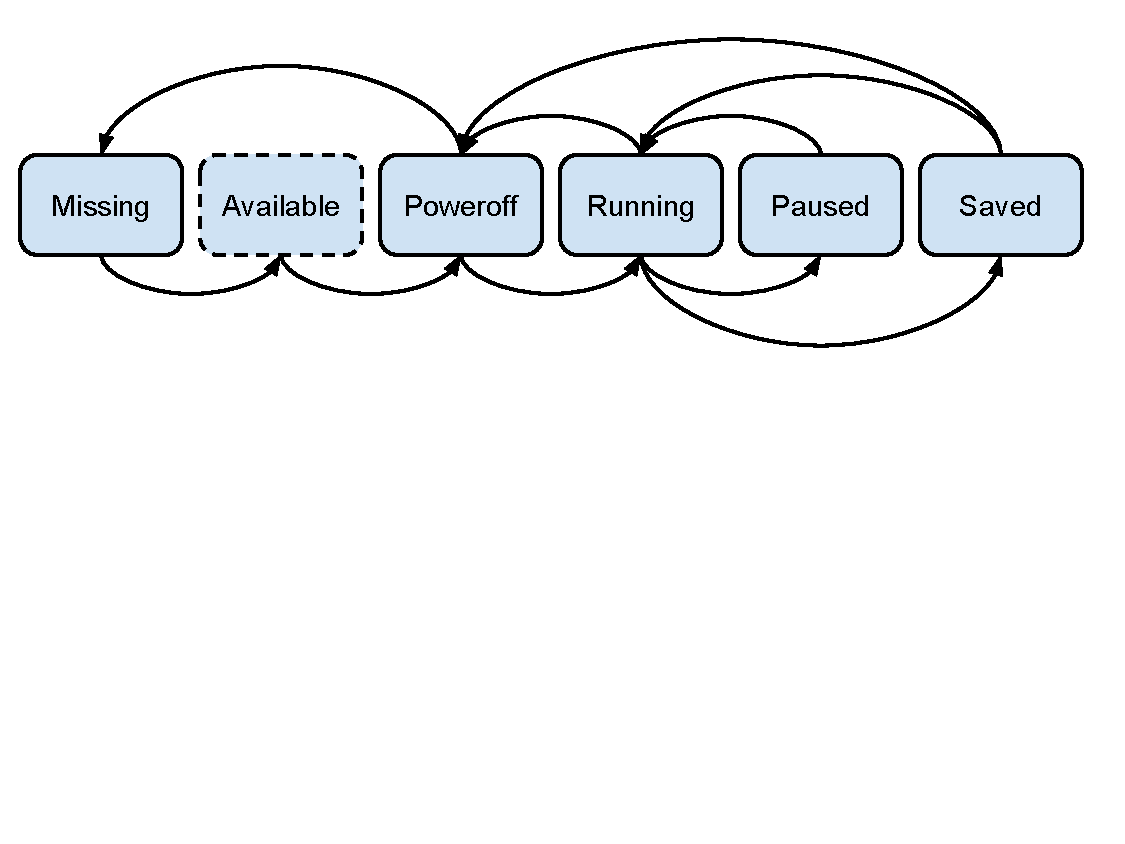
\includegraphics[width=\columnwidth]{imgs/webAPIEvents.pdf}
%  \end{center}
%\caption{xxx}
%\label{xxx}
%\end{figure}
%
%
%When the path of actions is completed and the FSM settles on a target state, the following events are fired:
%
%\begin{itemize}
%    \item {\bf vm.missing}: the VM does not exist.
%    \item {\bf vm.available}: the VM is defined in virtualbox but not yet configured.
%    \item {\bf vm.poweroff}: The VM is properly configured and powered off.
%    \item {\bf vm.saved}: the VM process has stopped and the state is saved to disk (hibernation)"
%    \item {\bf vm.paused}: the VM process is running yet it’s CPU is halted (paused in-memory).
%    \item {\bf vm.running}: the VM is running.
%\end{itemize}
%
%In addition, two special events are fired providing a higher-level information regarding the application that runs inside the Virtual Machine:
%
%\begin{itemize}
%\item {\bf vm.booted}: this event is fired when WebAPI fires the callback apiStateChanged(true), meaning that the designated port which is used for API communication between the javascript interface and the VM is available. We are assuming that the VM is “booted” because the port will be opened after the boot sequence is completed.
%
%{\textit NOTICE: This event might oscillate, because changes in the network connectivity (ex. user closing the laptop lid) will interrupt the communication, causing this event to be fired again when the network connectivity is resumed.}
%
%\item {\bf vm.collisions}: when through the API port, the javascript interface identifies that collisions are happening.
%
%{\textit NOTICE: This event has similar oscillations to vm.booted. That’s because the javascript interface is probing the job status through the API port. If the API port becomes unavailable, the interface will assume that there are no more jobs being processed. Therefore the instant it becomes available again (vm.booted), this event will be fired again.}
%
%\end{itemize}
%
%
%\subsubsection{Sequence of events}
%
%Since all these events are produced by the state changes of the FSM, they can only appear in sequences. The usual flow of events is shown on the following diagram:
%
%\begin{figure}[t]
%  \begin{center}
%		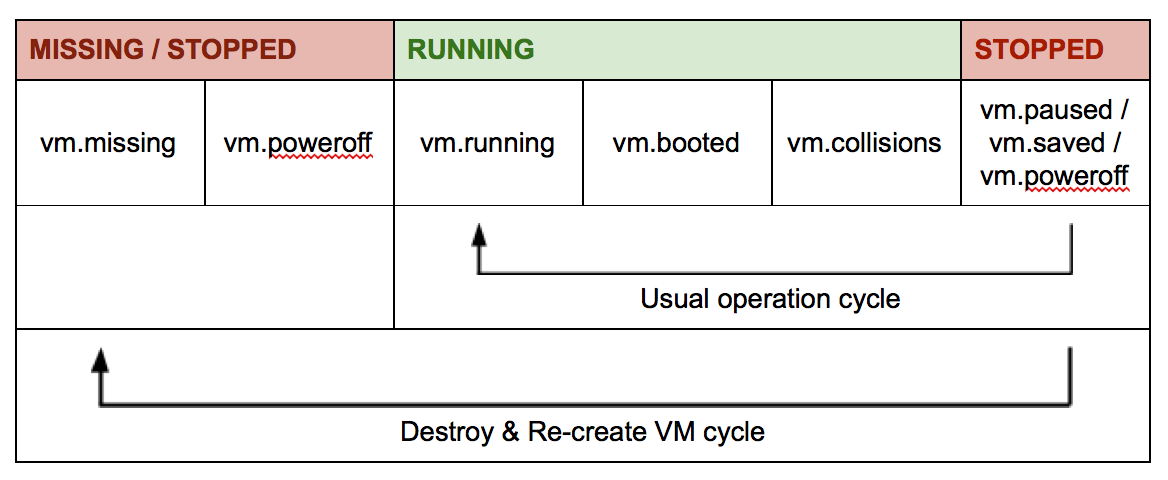
\includegraphics[width=\columnwidth]{imgs/sequenceOfEventsTable.png}
%  \end{center}
%\caption{xxx}
%\label{xxx}
%\end{figure}
%
%
%
%Therefore, you can extract some useful information:
%
%\begin{itemize}
%\item {\bf How long the VM was running?}: sum the differences in timestamps between the event "vm.running" and ANY of the following three events: "vm.paused", "vm.saved", "vm.poweroff"
%
%\item {\bf Did the user successfully manage to start a simulation?}: Check if AT LEAST one "vm.booted" event is fired after the “vm.running” event.
%\end{itemize}
%
%
%\subsubsection{User Events}
%
%These events are fired by user actions on the user interface. These are:
%
%\begin{itemize}
%    \item {\bf actions.open\_rdp}: user clicked on the "eye" icon that opens the console window. There the user can see the status of the job and the job manager.
%    
%    \item {\bf actions.open\_web}: user clicked on the "pop-out" icon that opens the website served from within the Virtual Machine. There the user can see the histograms produced by the current simulation
%actions.remove: User clicked on the trash icon which is going to remove the virtual machine from his/her computer.
%    \item {\bf actions.start}: user clicked on the “start” button, which is going to create, set-up and boot the VM. If the VM is already in any other state it will be switched to ‘running’ by following the path in the FSM diagram.
%    \item {\bf actions.stop}: user clicked on the “stop” button, which is going to SAVE the Virtual Machine to the disk (hibernate). 
%    \item {\bf actions.apply}: user clicked on the “apply” button, which is going to apply the changes (s)he did on the CPU/RAM.
%    \item {\bf actions.login}: user logged in with his/her social profile
%    \item {\bf actions.logout}: user disconnected his/her social profile
%\end{itemize}
%
%
%\subsubsection{Sequence of events with WebAPI}
%
%Most of the events fired by the WebAPI are triggered by the user. The following table shows which WebAPI events can a user event trigger. The events not included in the following table are not causing changes to the Virtual Machine.
%
%If you notice a sequence of events not matching the ones below, then the state change of the VM was most probably triggered by an external cause. 
%
%
%\begin{figure}[t]
%  \begin{center}
%		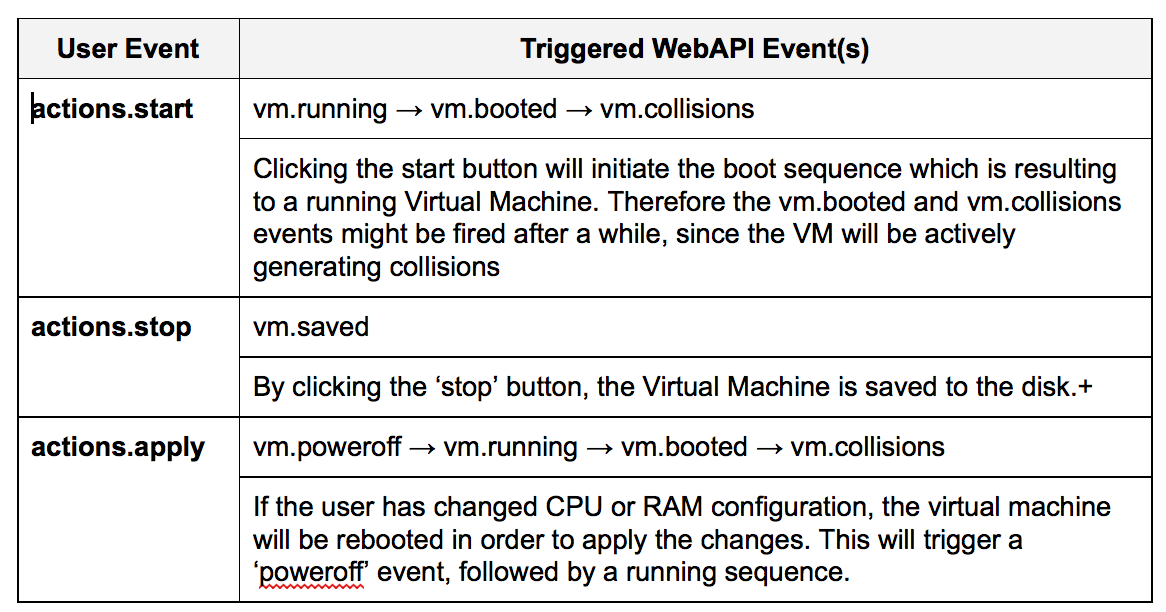
\includegraphics[width=\columnwidth]{imgs/webAPIEventsSequenceTable.png}
%  \end{center}
%\caption{xxx}
%\label{xxx}
%\end{figure}
%
%
%
%\subsubsection{Other user actions that could trigger WebAPI events}
%
%Since the user can still control the Virtual Machine without the Challenge Interface (ex. through VirtualBox), a state change can occur without a user-triggered action.
%
%
%\begin{figure}[t]
%  \begin{center}
%		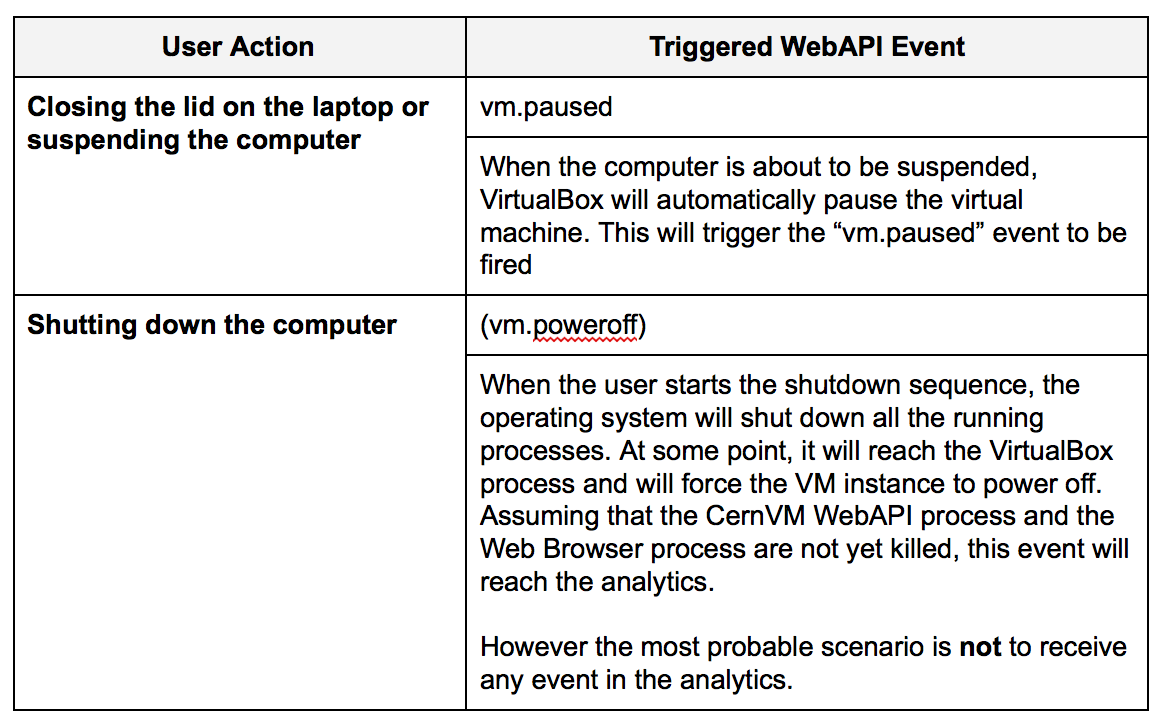
\includegraphics[width=\columnwidth]{imgs/userActions-webAPIEventsTable.png}
%  \end{center}
%\caption{xxx}
%\label{xxx}
%\end{figure}
%
%
%
%
%
%
%
%% \begin{itemize}
%% \item Briefly describe all projects using CCLtracker, Geotagx, VAS, 1st and 2nd CERN Challenges.
%% \item Focus on CERN challenges showing some examples of the data we gathered. 
%
%% \item It would be good to relate this data with the advantages we wrote in related work. 
%
%%  e.g. debugging tools --> Trace of errors combined with browsers, OS, device, etc..
%%       Knowing who are they --> Different segments and demographic information
%      
%%       Knowing their engagement --> picture about engagements. 
%      
%%       etc...
%
%% \end{itemize}
%